%chapter 4 discussion
\chapter{Discussion}
\label{sec:diss}
\chaptermark{Discussion}

\section{Other Multidimensional Scaling techniques with noise}
\label{D}

In \citet{Athreya2016} and \citet{OMNI}, the authors prove that adjacency spectral embedding of the random dot product graph gives rise to a central limit theorem for the estimated latent positions. In this work we extend these results to the previously unexplored area of perturbation analysis for CMDS, addressing a gap in the literature as acknowledged in \citet{Fan} and \citet{Peterfreund&Gavish}. Notably, the three noise models we proposed in Section \ref{sec:M&E} each give rise to a central limit theorem; that is, for Euclidean distance matrix, the rows of the configuration matrix given by CMDS under noise will center around the corresponding rows of the true configuration matrix. Furthermore, our simulations on the synthetic data together with the shape clustering data all demonstrated the validity of our results. We have avoided any discussion of the model selection problem of choosing a suitable embedding dimension $\hat{d}$. Instead, we assume $d$ is known -- except in Section 4.2. There are many methods for choosing (spectral) embedding dimensions, see \cite{Zhu&Ghodsi, Jackson, Chatterjee}. 

\begin{figure}[tp]
    \centering
    \subfloat[$n$=50]{{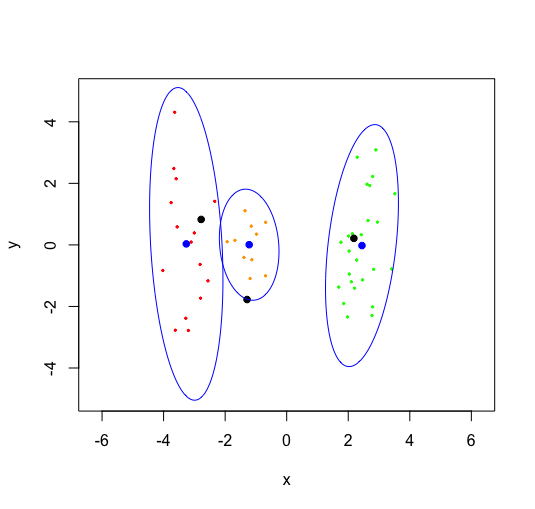
\includegraphics[width=.4\textwidth]{./figure/Uncommon_var_E_n_50.png} }}
    \quad
    \subfloat[$n$=100]{{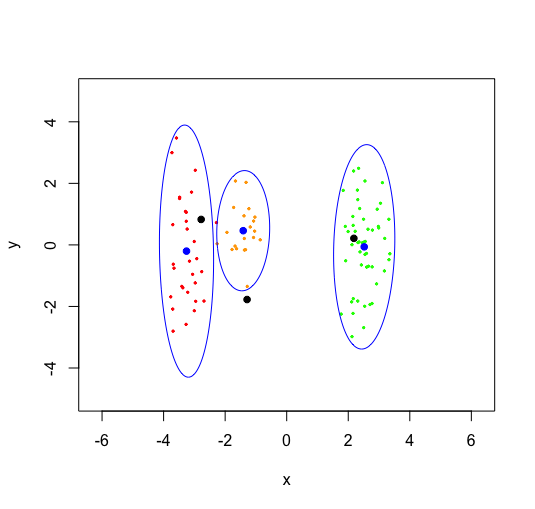
\includegraphics[width=.4\textwidth]{./figure/Uncommon_var_E_n_100.png} }}
    \quad
    \subfloat[$n$=500]{{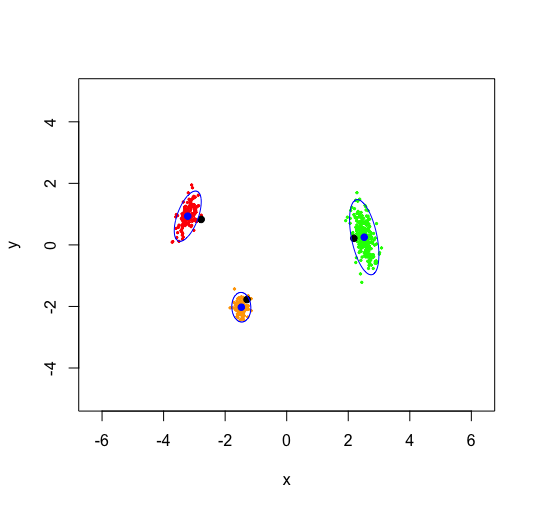
\includegraphics[width=.4\textwidth]{./figure/Uncommon_var_E_n_500.png} }}
    \quad
    \subfloat[$n$=1000]{{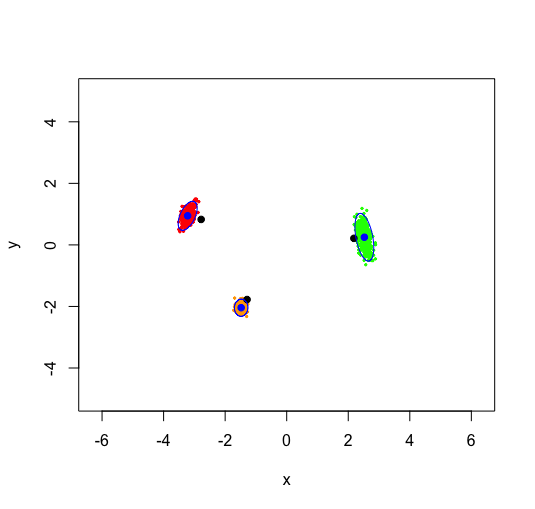
\includegraphics[width=.4\textwidth]{./figure/Uncommon_var_E_n_1000.png} }}
    \caption{Simulation of CMDS with heteroscedastic noise $\widetilde{E}$. The black dots are the true positions for the three points. The blue dots are the empirical means and the blue ellipses are the 95\% level curve of the empirical covariance matrix. Note that $\widetilde{E}$ used in this simulation is of the same order for the off-diagonal blocks as that used in Figure \ref{fig:Simulation result}. NB: there is asymptotic bias.}
    \label{fig:Uncommon_var_E}
\end{figure}

A practically relevant and conceptually illustrative example comes from relaxing the assumption of common variance for the entries of the noise matrix $E$ in Section \ref{D+E}: the consistency result from Theorem \ref{main_theorem_D+E} no longer holds. To illustrate this point, we return to our three-point-mass simulation presented in Section \ref{SD} and modify our noise model as follows: Let $\widetilde{E}_{ij} \iid \textrm{Uniform}(-D_{ij}, +D_{ij})$ for $i < j$ and $\widetilde{E}_{ij}= \widetilde{E}_{ji}$. (The noise now depends on the entries of $D$, and $\Delta = D + \widetilde{E}$ no longer has negative entries.) The embedding of $\Delta$ into two dimensions gives class-conditional Gaussians; however, we have introduced bias into the embedding configuration. Figure \ref{fig:Uncommon_var_E} shows, for one realization, the embedding result. Note that the empirical mean and the theoretical positions do not coincide in simulation with large $n$, and theoretically even in the limit.
\begin{figure}[tp]
    \centering
    \subfloat[$n$=50]{{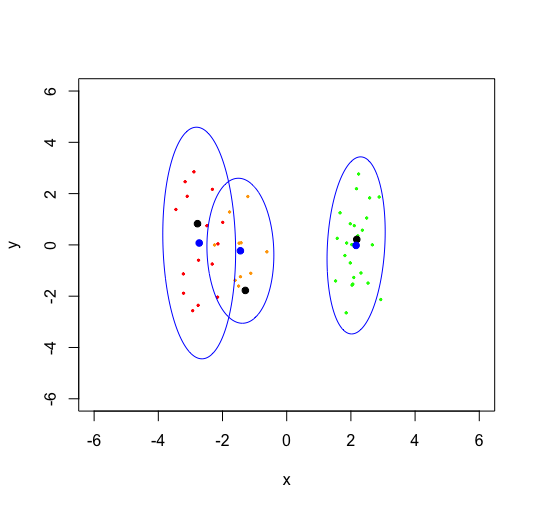
\includegraphics[width=.4\textwidth]{./figure/raw_stress_n_50.png} }}
    \quad
    \subfloat[$n$=100]{{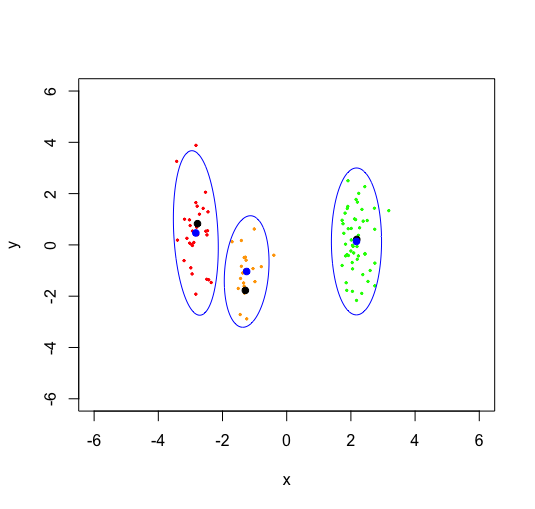
\includegraphics[width=.4\textwidth]{./figure/raw_stress_n_100.png} }}
    \quad
    \subfloat[$n$=500]{{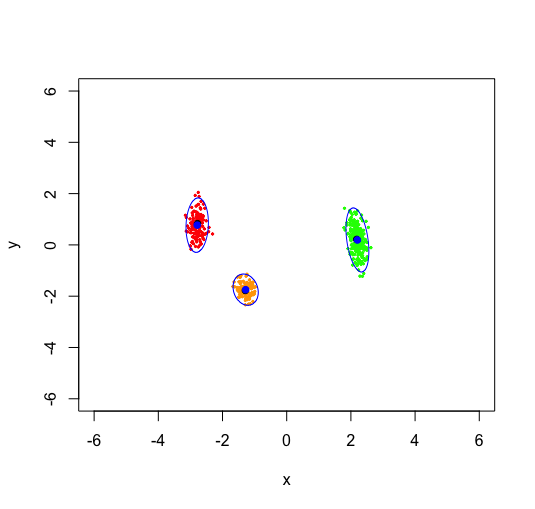
\includegraphics[width=.4\textwidth]{./figure/raw_stress_n_500.png} }}
    \quad
    \subfloat[$n$=1000]{{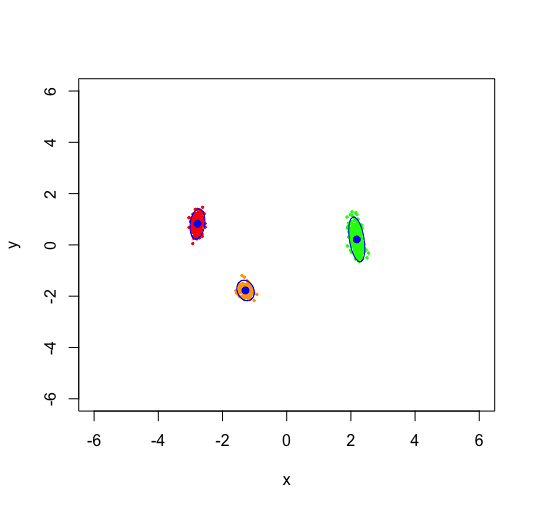
\includegraphics[width=.4\textwidth]{./figure/raw_stress_n_1000.png} }}
    \caption{Simulation of MDS using raw stress criterion for $n$=50, 100, 500 and 1000 points.
                  The black dots are the true positions of $x_1$, $x_2$ and $x_3$, the blue dots are the empirical mean of the simulation and the blue ellipses are the 95\% level curve of the empirical covariance matrix.}
    \label{fig:RawStress}
\end{figure}

CMDS is just one of a wide variety of multidimensional scaling techniques. Minimizing the raw stress criterion is another commonly used MDS technique \citep{Leeuw-Heiser}, i.e., given a $n \times n$ observed dissimilarity matrix $\Delta$ and an embedding dimension $d$, one seeks to minimize the objective function $$\sigma_r = \sigma_r(X) = \sum\limits_{(i,j)} (\delta_{ij} - \|X_i - X_j\|)^2.$$ The minimization of $\sigma_r(X)$ is with respect to all configurations $X \in \mathbb{R}^{n \times d}$ and usually proceeds via an iterative algorithm which updates the configuration matrix $X$ until a stopping criterion is met. Keeping the simulation settings as in Section \ref{SD},  the resulting configuration is shown in Figure \ref{fig:RawStress}. This suggests that the CLT may hold for raw stress just as well as for CMDS. However, this claim is at best a conjecture at present as perturbation analysis of stress minimization algorithms is significantly more involved.
%%%%%%%%%%%%%%%%%%%%%%%%%%%%%%%%%%%%%%%%%%%%%%%%%%%%%%%%%%%
\section{Conjecture: CMDS on Omni Embedding of graphs and Hypothesis Testing}
Given a collection of Random Dot Product Graphs: $A^{(1)}, A^{(2)}, \ldots, A^{(m)}$, each with $n$ vertices, \cite{OMNI} seeks to jointly embed all $m$ graphs into a common (prespecified) $d$-dimensional Euclidean space by embedding the $nm \times nm$ OMNI Matrix $\mathcal{M}$ given by
$$
\mathcal{M} :=
\begin{bmatrix}
     A^{(1)}       & \frac{A^{(1)} + A^{(2)}}{2} & \frac{A^{(1)} + A^{(3)}}{2} & \dots & \frac{A^{(1)} + A^{(m)}}{2} \\
    \frac{A^{(2)} + A^{(2)}}{2}     & A^{(2)} & \frac{A^{(2)} + A^{(3)}}{2} & \dots & \frac{A^{(2)} + A^{(m)}}{2} \\
    \vdots & \vdots & \vdots & \ldots & \vdots \\
    \frac{A^{(m)} + A^{(1)}}{2} & \frac{A^{(m)} + A^{(2)}}{2} & \frac{A^{(m)} + A^{(3)}}{2} & \dots & A^{(m)}
\end{bmatrix}.
$$
Using the notation in \cite{OMNI}, let $S_\M$ represent the $d \times d$ matrix of top $d$ eigenvalues of $\M$, ordered by magnitude, and let $U_\M$ be the $mn \times d$-dimensional matrix of associated eigenvectors. Define the omnibus embedding, denoted OMNI($\mathcal{M}$), by $U_\M S^{1/2}_\M$, note that OMNI($\mathcal{M}$) produces $m$ separate points in Euclidean for each graph vertex, effectively one such point for each copy of the multiple graphs in our sample. Furthermore, denote 
\begin{equation}
    U_\M S^{1/2}_\M =
\begin{bmatrix}
     \hat{X}^{(1)}\\
     \hat{X}^{(2)}\\
     \vdots \\
     \hat{X}^{(m)}
\end{bmatrix}
\end{equation}
where each $\hat{X}^{(i)}$ is an $n \times d$ matrix representing the embedding of the $i$th random graph in $d$ dimension. 

As pointed out in \cite{OMNI}, the omnibus embedding introduces alignment between graphs by placing an average on the off-diagonal blocks of $\M$, merely considering a Frobenius norm difference between blocks of the omnibus embedding 
$\| \hat{X}^{(i)} - \hat{X}^{(j)} \|_{F}$
without any Procrustes alignments provides meaningful discrimination between graphs with different latent positions. Specifically, we can construct an $m \times m$ distance matrix $\Delta$ given by $\Delta_{ij} := \| \hat{X}^{(i)} - \hat{X}^{(j)} \|_{F}$ as an estimation for the Frobenius distance matrix $D$ between true latent positions $ D_{ij} := \| X^{(i)} - X^{(j)} \|_{F}$, where $X^{(i)}$ is the true latent position for the $i$th graph. That is, $\Delta = D + E $ for some $m \times m$ noise matrix $E$. \textcolor{red}{(Note that the entries of $E$ are correlated. Furthermore, $\mathbb{E}[E] = 0$ only when all the $m$ graphs shares the same underlying true latent position. Those two observations make the proof of the following conjectures quite a bit more challenging).}

A natural thing to do now is to perform classical multidimensional scaling (CMDS) on $\Delta$ and $D$ and compare the resulting configuration matrix $\hat{\G}$ = CMDS($\Delta$) and $\G$ = CMDS($D$), and we propose the following conjecture:
\begin{Conjecture}
Using the above notations, we propose:
$$ \lim_{m {\to} \infty} \mathbb{P} \{\sqrt{m} [(\hat{\G}W_m)_i - (\G)_i ]\leq \alpha\} = \int_{supp \textrm{F}} \Phi(\alpha, \Sigma(\emph{z})) dF(\emph{z}) $$ where $z$'s depends on the true underlying distribution of the latent positions $X$ of the graphs.
\end{Conjecture}
